\subsection{Optical Tracking}
It is possible to locate an object using an optical sensor. This work by converting a change in light into a electric signal, that is measured and compared to a reference signal. 

Because of weather related issues, optical tracking of a drone might not be a functional solution. If the drone is behind clouds or simply is unrecognizable by the optical sensor, due to weather conditions like rain, snow or a fog, the optical tracking is not working. 

Because of these issues optical tracking is rejected. 

\subsection{\glsentrylong{aoa} determination from signal distance difference}\label{sec:detSignalDistanceDifference}
Signal difference is based on the fact, that if the drone is sending out a beacon signal, the distance the signal has to travel to reach two  different antennas on the ground is different. This difference in distance can be used to determine the \gls{aoa} of the signal. This signal difference can be determined in many different ways, in this subsection three different methods is explained and later in \autoref{subsec:SignalStrengthPathLossMethod} a third method is explained as well. 

All the methods using signal difference need a setup with two or more receiving antennas. For simplicity two antennas receiving setup is assumed in order to explain the functionality of the different methods. Such a receiver setup is seen on \autoref{fig:RSSI_tracking}. 
\begin{figure}[h]
	\centering
	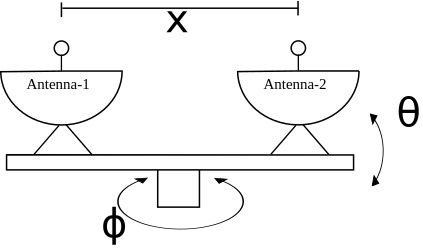
\includegraphics[width=0.6\linewidth]{AntennaSetupSeenFromAbove}
	\caption{Placement of tracking antennas in a signal difference tracking system, seen from above.}
	\label{fig:RSSI_tracking}
\end{figure}

The formula for determining the \gls{aoa} can be derived using geometry.
Considering a signal sent from the drone at point $P$ on \autoref{fig:phase_drawing}, two antennas are placed at respectively at $S_1$ and $S_2$. The paths that the signal travels to reach the two antennas are $d_1$ and $d_2$. At the point $M$ the signal has travelled the same distance.
The difference in length the signals have to travel is denoted $y$ and is equal to $d_1-d_2$. 
\begin{figure}[h]
\centering
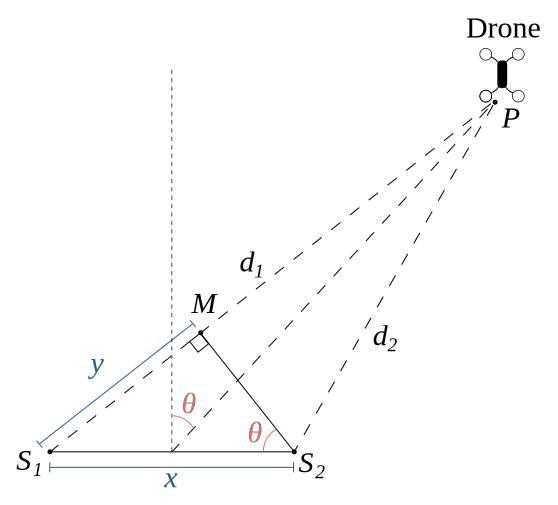
\includegraphics[width=0.7\linewidth]{Phase/Phase_drawing}
\caption{Illustration of determination of \gls{aoa} using signal distance difference. P is the point where the drone is located. $d_1$ and $d_2$ are the respective distances between the drone and the two receiving antennas $S_1$ and $S_2$. The distance between the antennas is $x$ and the difference of $d2$ and $d_1$ is y. $M$ denotes the point where the two distances are equal. The \gls{aoa} is approximately $\theta$ when $d_1 \gg x$ and $d_2 \gg x$.}
\label{fig:phase_drawing}
\end{figure}

The \gls{aoa}, $\theta$, can be calculated using trigonometry. It is assumed that the sender $P$ is so far away, so that from the two antennas point of view the drone is a plane instead of a point. This allows the approximation that the two lines, $d_1$ and $d_2$, can be considered parallel.
This means that the angle $\theta$ at $S_2$, also becomes the \gls{aoa} which can be calculated using sine \citep{TechReport:DirectionFindingPaper}.

The \gls{aoa} can then be calculated with \autoref{eq:aoa_general}. 
\begin{equation} \label{eq:aoa_general}
	\theta = \arcsin\left(\frac{y}{x}\right) \addunit{\radian}
\end{equation}
\startexplain
\explain{$\theta$ is the \gls{aoa}}{\si{\radian}}
\explain{$y$ is the physical distance difference, between each of the receivers and the drone}{\si{\meter}}\explain{$x$ is the spacing between the two antennas}{\si{\meter}}
\stopexplain

The method described above is only be able to measure \gls{aoa} within a \SI{180}{\degree} field of view since two mirrored points result in the same distance, $y$. 
This can be seen on \autoref{fig:phase_double}. To avoid this ambiguity, $y$ has to be measured with more than two receivers \citep{TechReport:Amundson2010}. In this report for the sake of simplicity only a two antennas setup is considered.
\begin{figure}[h]
\centering
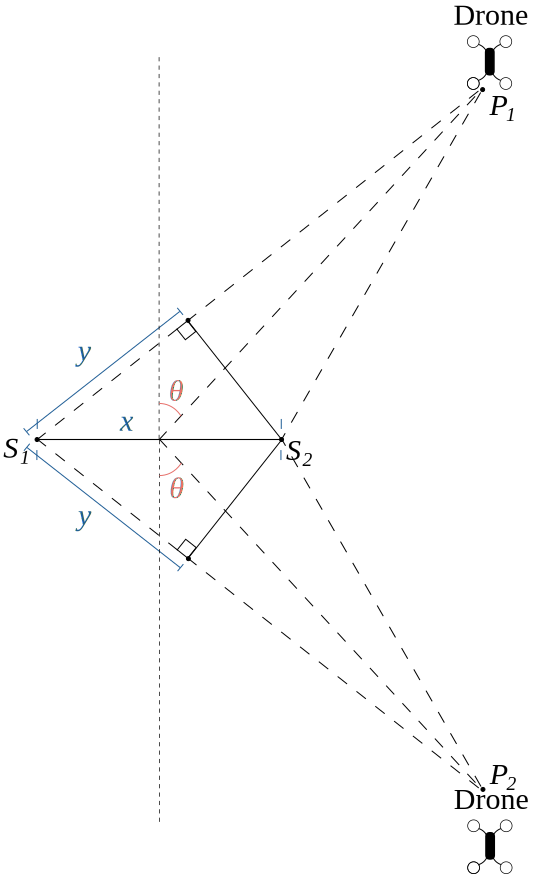
\includegraphics[width=0.4\linewidth]{Phase/phase_double}
\caption{The two points $P_1$ and $P_2$ result in the same signal characteristics being measured at the receivers $S_1$ and $S_2$. This means that a two antenna system only have a field of view of \SI{180}{\degree}}.
\label{fig:phase_double}
\end{figure}

\newpage
Three method using \gls{aoa} is analysed in this report:
\begin{itemize}
	\item Time of arrival 
	\item Phase difference detection 
	\item Signal strength difference
\end{itemize}

\subsubsection{\glsentrylong{toa}} \label{TimeOfArrival}
With this method a receiver setup as the one explained on \autoref{fig:RSSI_tracking} is assumed. In this case the drone emits a impulse signal whenever the position of the drone is needed. If the drone moves, a new impulse must be emitted in order for the ground station to know the new location of the drone.

The \gls{toa} method uses the time difference in reception of a source between two receivers. The finite speed of electromagnetic wave propagation causes a time difference between the reception time on two antennas when the signal source is not placed at exactly the same distance to each antenna.

The difference of time between the moment each antenna receives the signal multiplied with the speed of light, represents the difference in distance between the drone and each of the two antennas. That way the distance difference, $y$ from \autoref{eq:aoa_general}, can be determined by: 
\begin{equation} \label{eq:LenghtDifference}
		y = \Delta t \cdot c \addunit{\meter} 
\end{equation}
\startexplain
\explain{$\Delta t$ is the time difference between the two antennas reception of the signal}{\si{\second}}
\explain{$c$ is the speed of light}{\si{\meter \per \s}}
\stopexplain

Combining \autoref{eq:LenghtDifference} and \autoref{eq:aoa_general} yields \autoref{eq:actualLenghtDifference}. 
\begin{equation} \label{eq:actualLenghtDifference}
	 \theta = \arcsin \left( \frac{ \Delta t \cdot c}{x} \right) \addunit{\radian}
\end{equation}

If the difference in time is not registered and measured correctly the calculated angle deviate from reality. In \autoref{sec:RequiredPrecision} it was found that the allowed error in the tracking should be less than \SI{2,08}{\milli\radian}. By inserting the value of the allowed error combined with the assumption that the distance between the antennas is 20 cm into \autoref{eq:actualLenghtDifference} yield: 
\begin{subequations}
\begin{align}
\theta &= \arcsin \left( \frac{\Delta t \cdot \SI{300 000 000}{\meter\per\second} }{\SI{200}{\milli\meter}} \right) =  \SI{2,08}{\milli\radian} \label{eq:TOA:eq3} \\
\Delta t &= \SI{1,3867}{\pico\second} \label{eq:TOA:eq4}
\end{align}
\end{subequations} 

From \autoref{eq:TOA:eq4} it is seen that a measuring error of \SI{1,3867}{\pico\second} equals to the maximum allowed angular deviation. From this it can be deduct that the signal at the two receivers should be sampled much faster than $\frac{1}{\tau_{error}} = \frac{1}{\SI{1.3867}{\pico\second} } = 721 \si{\giga\hertz}$

For this project a sampling frequency of more than \SI{721}{\giga\hertz} is not possible for a digital implementation, as such it was decided to not pursue the research further.

\subsubsection{Phase difference detection} \label{PhaseDifferenceDetection}
With this method a receiver setup as the one explained on \autoref{fig:RSSI_tracking} is assumed. For this method the drone should emit a continuous wave signal. 

The distance difference $y$ from \autoref{eq:aoa_general}, can be determined by measuring the phase difference of the signal at the two antennas. Thus the difference in distance can be expressed by \autoref{eq:phasedaoay}. 
\begin{equation} \label{eq:phasedaoay}
y=\frac{\lambda\cdot\Delta\varphi}{2\pi} \addunit{\meter}
\end{equation}
\startexplain
\explain{$\lambda$ is the wavelength of the signal}{\si{\meter}}
\explain{$\Delta\varphi$ is the phase difference of the signal between the two antennas}{\si{\radian}}
\stopexplain

When isolating \autoref{eq:phasedaoay} for $\Delta\varphi$ the equation becomes \autoref{eq:phasedaoayV2}. 
\begin{equation} \label{eq:phasedaoayV2}
\Delta\varphi=y \cdot \frac{2\pi}{\lambda} \addunit{\radian}
\end{equation}

In practice when measuring the phase difference of the two signals it falls in the interval: $-\pi<\Delta\varphi<\pi$. Therefore it can be seen from \autoref{eq:phasedaoayV2}, that $y$ must fall in the interval $\frac{-\lambda}{2} < y < \frac{\lambda}{2}$. This relation can be ensured if the distance between the antennas is $\frac{\lambda}{2}$. This avoids phase ambiguity \citep{TechReport:DirectionFindingPaper,TechReport:Amundson2010}. 

The maximum phase difference occur when the sender is located collinear with the receiver. If the \gls{aoa} is directly above the two receiving antennas, the phase difference is \SI{0}{\radian}.

From \autoref{eq:aoa_general} and \autoref{eq:phasedaoay} the \gls{aoa} when using the phase difference becomes as descried by \autoref{eq:GeneralPhaseDelayEquation}. 
\begin{equation} \label{eq:GeneralPhaseDelayEquation}
	\theta = \arcsin\left(\frac{\frac{\lambda\cdot\Delta\varphi}{2\pi}}{x}\right) \addunit{\radian}\\
			   = \arcsin\left(\frac{\lambda\cdot\Delta\varphi}{2\pi x}\right)\addunit{\radian}
\end{equation}
\startexplain
\explain{$x$ is the distance between the antennas}{\si{\meter}}
\stopexplain

Errors in the \gls{aoa} reading occurs depending on the \gls{snr} of the signal, this error is defined by \autoref{eq:phase_doa_error} \citep[p. 43]{book:shinohara}. 
\begin{equation} \label{eq:phase_doa_error}
\Delta\theta ' = \frac{\lambda}{\pi x \cos(\varphi) \sqrt{\text{SNR}}} \addunit{\radian}
\end{equation}
\startexplain
\explain{$\Delta\theta '$ is the error of \gls{aoa} estimation}{\si{\radian}}
\explain{SNR is \glsentrylong{snr}}{1}
\stopexplain

From \autoref{eq:phase_doa_error} it is clear that the spacing of the antennas should be as large as possible to achieve the lowest \gls{aoa} estimation error. The maximum possible distance is $\frac{\lambda}{2}$ as described earlier in this section.

\cite{TechReport:DirectionFindingPaper} defines a worst case \gls{snr} of their tracking system to be \SI{20}{\decibel} and a best case \gls{snr} of \SI{60}{\decibel}.


A required precision was found in \autoref{sec:RequiredPrecision} \autoref{eq:RequiredPrecision}, to be better when \SI{2.08}{\milli\radian}. This means that a \gls{snr} of \SI{20}{\decibel} is not tolerable. 
To calculate the lowest tolerable \gls{snr}, values are inserted into \autoref{eq:phase_doa_error} this yields that  the lowest tolerable \gls{snr} should be above \SI{46.7}{\decibel} to achieve a precision of \SI{2.08}{\milli\radian} based on the calculated in \autoref{eq:phase_reqsnr}.
\begin{subequations} \label{eq:phase_reqsnr}
	\begin{align}
	\text{SNR} 	&> 10 \log_{10}\left(\frac{\lambda^2}{\pi^2x^2\cos(\varphi)^2\theta_{min}^2}\right) \addunit{\decibel}\\
			    &> 10 \log_{10}\left(\frac{2}{\pi^2\cos(0)^2 \cdot (\SI{2,08}{\milli\radian})^2}\right) \si{\decibel}\\
			    &> \SI{46.7}{\decibel}
	\end{align}
\end{subequations}

The \gls{snr} is a measure of the signal strength of the received signal compared to the signal strength of the noise. 

The \gls{snr} can be increased if more antennas are used, therefore more precise \gls{aoa} estimations are usually made with an array of receivers \citep{book:shinohara}. Another way to increase the \gls{snr}, is simply to increasing the received signal strength by transmitting with more power. 

The phase detection method has good potential, but the precision depends on the received power. 

\subsection{Signal strength difference} \label{SignalStrengthDifference}
Another way to determine the \gls{aoa} of a drone is to have the target drone emit a signal, whenever it wants to be tracked. The pilot signal is captured with a two antenna setup like the one seen on \autoref{fig:RSSI_tracking}. The strength of the two received signal are compared and used to locate the drone. This is known as \gls{rssi} tracking. 

%Another way to determine the \gls{aoa} of a drone is to compare the strength of a pilot signal that the targeted drone emits when it wants to be tracked. This is known as \gls{rssi} tracking. 
%%Assuming the drone is transmitting a pilot signal, that is collected by a  minimum two tracking antennas, these antennas should have a physical distance between them.  
%The strength of the signal emitted by the drone should be captured in two or more antennas, in order to compare the the signals. The antennas should be have a physical distance between them. 

The signal strength difference can be used in different ways to track the drone, some of the methods is analysed in this section. 

\subsubsection{Continuous tracking with closed feedback loop controller}
One method to find the direction of the drone is to have a two antenna setup as on \autoref{fig:RSSI_tracking}. 
The two antennas should continuously measure the signal strength of the incoming signal. The difference in received signal strength between the two tracking antennas is compared and treated as an error signal in a closed loop feedback controller. 

The stand rotate according to the signal strength of the two antennas. If the signal is strongest on the left antenna, then the antenna stand would rotate left, and vice versa.

By having this continuous tracking the antenna stand rotate until the signal strength of the pilot signal is equally strong on both of the tracking antennas, which is the case when the antenna stand is pointing directly at the drone. 

The method is simple and precise enough for many uses. However to increase the precision many factors have to be considered, including the directivity of the tracking antennas, the gain difference between the antennas and the reflections. 

\subsubsection{Signal strength path loss method}\label{subsec:SignalStrengthPathLossMethod}
Another method to find the drone with the setup shown on \autoref{fig:RSSI_tracking}, is to map \gls{rssi} to distance using the path loss method. For this method the drone needs to emit a signal as well, but in this case the shape of the signal is not important, it could both be an impulse or a continuous wave.

It is known that the signal strength is decreasing as the wave front travels trough free space. The equation for free space path loss is \autoref{eq:SSLossPath}, which is also a simplified version of Friis Transmission Equation (assuming two isotropic antennas in free space without any gain).
\begin{equation} \label{eq:SSLossPath} 
L = 20 \cdot \log10\left(\frac{4\pi\cdot d}{\lambda}\right) \addunit{\decibel}
\end{equation}
\startexplain
\explain{$L$ is the path loss}{\si{\decibel}}
\explain{$\lambda$ is the wavelength of the signal}{\si{\meter}}
\explain{$d$ is the distance between the antenna and the drone}{\si{\meter}}
\stopexplain

The path loss can be calculated if the power transmitted and the power received is known as seen in \autoref{eq:simplepathloss}
\begin{equation} \label{eq:simplepathloss}
L = 10\log10\left(\frac{P_R}{P_T}\right)  \addunit{\decibel}
\end{equation}
\startexplain
\explain{$L$ is loss}{1}
\explain{$P_T$ is the transmitted power}{\si{\watt}}
\explain{$P_R$ is the received power}{\si{\watt}}
\stopexplain

With \autoref{eq:SSLossPath} the distance from the receiving antenna to the transmitting antenna can be found with \autoref{eq:SSLossPathDistance} (Note that this is the distance from the drone to one of the receiving antennas). 
\begin{equation} \label{eq:SSLossPathDistance} 
d = \frac{\lambda}{4\pi} \cdot 10^{\frac{L}{20}} \addunit{\si{\meter}}
\end{equation}

If the distance from the drone to both the receivers is known, then basic trigonometry can be used to find the direction of the drone. The needed trigonometric calculations is the same as the ones used to utilize the signal distance difference method in \autoref{sec:detSignalDistanceDifference}, therefore the \gls{aoa} can be determined from \autoref{eq:aoa_general}. 

With this method the distance difference, $y$ (seen on \autoref{fig:phase_drawing} and in \autoref{eq:aoa_general}), can be calculated from the difference in distance to the drone. This is done by inserting \autoref{eq:SSLossPathDistance} into \autoref{eq:SSLossPathAngle1} which yields \autoref{eq:SSLossPathAngle2}. 
\begin{align}
y &= | d_{a1} - d_{a2} | \addunit{\meter} \label{eq:SSLossPathAngle1} \\
  &= \frac{\lambda}{4\pi} \cdot \left| 10^{\left(\frac{L_{a1}}{20}\right)} - 10^{\left(\frac{L_{a2}}{20}\right)} \right| \addunit{\meter} \label{eq:SSLossPathAngle2}
\end{align}
\startexplain
\explain{$y$ is the distance difference from each of the antennas to the drone}{\si{\meter}}
\explain{$L_{a1}$ is the path loss of antenna 1}{\si{\decibel}}
\explain{$L_{a2}$ is the path loss of antenna 2}{\si{\decibel}}
\explain{$\lambda$ is the wavelength of the signal}{\si{\meter}}
\stopexplain

Combining \autoref{eq:aoa_general} and \autoref{eq:SSLossPathAngle2} yields the final equation:
\begin{equation} \label{eq:SSLossPathAngleFinal}
	\theta = \arcsin\left( \frac{\lambda}{4\pi \cdot x} \cdot \left| 10^{\left(\frac{L_{a1}}{20}\right)} - 10^{\left(\frac{L_{a2}}{20}\right)} \right|  \right) \addunit{\radian}
\end{equation}
\startexplain
\explain{$\theta$ is the \gls{aoa}}{\si{\radian}}
\explain{$x$ is the spacing between the two antennas}{\si{\meter}}
\stopexplain

In order for this method to work the fraction inside the arcsin should always be less than 1, as stated in \autoref{eq:SSLossPathAngleRule}, else the found angle becomes complex. 
\begin{equation} \label{eq:SSLossPathAngleRule}
\frac{\lambda}{4\pi \cdot x} \cdot \left| 10^{\left(\frac{L_{a1}}{20}\right)} - 10^{\left(\frac{L_{a2}}{20}\right)} \right| \leq 1
\end{equation}

If an error occurs and the signal strength is measured wrong, then the found \gls{aoa} is of course not exact.  Assuming a frequency of \SI{800}{\mega\hertz} and a distance between the antennas of \SI{20}{\centi\meter}. Then if the signal strength, in one of the antennas is measured with at error of \SI{3}{\decibel}, using \autoref{eq:SSLossPathAngleFinal} this means an error of \SI{691}{\milli\radian} in the found direction of the drone which is 300 times more that our allowed angular deviation. 

